\subsection{Methodology}

The methodology for each malware detection application is as follows.  For each
application, we will first present the malware detection model, including the
relevant external sensors and rules to the anomaly detection; then we perform
experiments and analysis to validate the feasibility of our models.

\subsubsection{Experimental Setup}
Our experimental setup consists
of one router and
several hosts connected by 100Mbps connections to the Internet
through the router. First, we gather normal data from three
uncompromised hosts for a period of 12 days. Next, we ``compromise''
one host by installing the modified Agobot on it and control it from
another machine. The compromised host carries out
different activities on demand: generate spam email, start a DDoS
attack and perform password cracking.
More experimental details are described in the relevant section.

Three types of sensor data are collected on the hosts: $(i)$
user presence; $(ii)$ CPU temperature; and $(iii)$ network traffic.
User presence is represented by a binary-valued time series,
indicating whether the user is sitting at the host.
We use infrared sensors to detect user presence.
This is more reliable compared
to using acoustic sensors to detect keyboard typing or mouse clicks.
One reason is that a user can be simply looking at the monitor and not
doing anything.
Another reason is that malware can fool the sensor by playing back clicks.

The CPU temperature measurement
is represented by a real-valued time series giving the
temperature at the processor, which correlates to CPU load. In
principle, the CPU temperature should be measured with a sensor
between the CPU heat sink and fan, but we had difficulty in doing so
with our sensor. As a proof of concept, we used the CPU
temperature obtained from the host's operating system as a
proxy.\footnote{We use the
system call \emph{IDebugDataSpaces--$>$ReadMsr}() in Windows.
}
We remark that the sensor data should be measured and sent to the
monitor via a secure channel, and thus our temperature readings
is only a simulation to simplify the experiments.
For network traffic, headers of all packets and partial payload
passing through the router are logged.

\subsubsection{Detection Methods}

We use three detection methods for each application in this section.  We then
demonstrate that the execution of malware can be detected using any of these
methods using our framework.  The three detection methods are rate based
detection, moving average detection, and changepoint detection (our modified
version of the CuSum algorithm).

\paragraph{Rate Based Detection}

The general idea is that the allowable usage rate is dependent on user presence.
When the user is present, the resource usage rate is higher than 
when the user is absent.

This metric limits the resource usage rate 
and uses an application specific threshold for detection.
The specific threshold for a particular application 
can be determined from normal usage profiles.

The main advantage of rate based detection is its simplicity. 
However, the drawback is that it is very sensitive to the instantaneous rate. 
Thus, it has potential in having a high false positive or false negative rate. 
In addition, the detection threshold is prone to tampering if it is adaptive.

\paragraph{Moving Average Detection}

The moving average of $x_i$ is defined by the formula below
\begin{equation}\label{movAvg}
    \overline{x_i} = \left\{ \begin{array}{lr}
        (\sum_{j=1}^{i}{x_j})/i, & 1 \leq i < n \\
        (\sum_{j=i-n+1}^{i}{x_j})/n, & i \geq n
    \end{array} \right.
\end{equation}
where $n$ is the number of readings taken into an average measurement. An
anomaly is detected at time $i$ if $\overline{x_i}$ exceeds a chosen threshold
that bounds the normal values.

%The detection threshold is placed on the moving average $\overline{x_i}$ at time $i$.
Arguably, moving average is less sensitive to the instant rate surge, thus it
reduces the amount of false positives as compared to rate based detection. If
the anomaly starts at time 1 or prior to the detection phase, the anomaly can
be detected in a similar time to the rate based detection. However, if normal
behavior is observed initially for some time, the alert of abnormal behavior is
delayed due to the averaging behavior.

\paragraph{Changepoint Detection}\label{subsec:changepoint}

\begin{table*}[tb]
  \centering
  \noindent\makebox[\textwidth]{%
  \begin{tabular}{|l|l|}
  \hline
  Malware Threat & Rules for triggering alarms \\
  \hline
  Email Spammer & (i) \ No user is present, and at least one email is sent; or \\
                & (ii) A user is present, and changepoint detection decides that \\
                & \hspace*{2em} the cumulative sum of email sent exceeds a threshold. \\
  \hline
  DDoS Zombie   & Changepoint detection detects the cumulative sum of the net \\
                & outgoing packet rate
        exceeds thresholds for user present and absent \\
  \hline
  Password Cracker & Changepoint detection detects the cumulative sum of \\
                   & CPU temperature exceeds a certain threshold
                   when user is absent  \\
  \hline
  \end{tabular}}
  \caption{Overview of malware detection rules using changepoint detection. }\label{tbl:detect-malware}
\end{table*}

The problem of changepoint detection~\cite{basseville1993detection} is to
detect changes from normal behavior.
We use a customized version of CuSum~\cite{page1954continuous} to do such
detection. In our model, behaviors are described as a real-valued
time series $x_1, \ldots, x_n$. Normal behavior is estimated to have a value
$a$ or smaller. To detect an
increase from the normal behavior,
the following cumulative sum $S_n$ is computed.
\begin{displaymath}
\left\{
\begin{aligned}
S_0 &= 0, \\
S_n &= S_{n-1} + \max(0, x_{n} - a), \ \ \ n \geq 1,
\end{aligned}
\right.
\end{displaymath}
\noindent where $x_n$ is the observation at time $n$ from the
sampling process. The value of $a$ can either be determined by the system
administrator, or by observing samples of normal behaviors to select
the smallest acceptable normal upper bound for $x_n$. If $S_n$
exceeds the threshold $N$, a change point is detected at time $n$
and the alarm will be triggered. Note that $a$ can be exceeded when
the normal behavior is violated, so $a$ is a lower detection threshold
for abnormal behavior, $S_n$ is the cumulative sum
of the actual signal and $N$ is the
changepoint detection threshold. CuSum can be shown to be optimal
under certain conditions \cite{basseville1993detection}. As it is simple
and efficient, it is suitable for real-time processing of streaming
sensor data.

\begin{figure}[tb]
\begin{center}
\begin{minipage}[t]{.49\textwidth}
     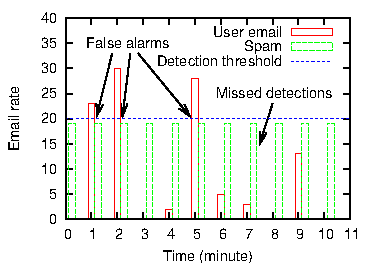
\includegraphics[width=1\textwidth]{sensor/email}
\vspace*{-4mm}
\caption{False detections caused by email rate based
spam detection}
\label{fig:detect-by-rate}
\end{minipage}
\begin{minipage}[t]{.5\textwidth}
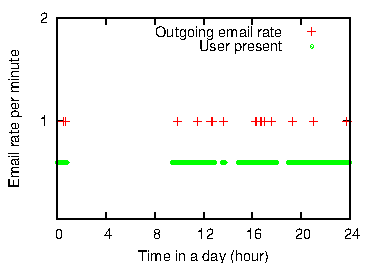
\includegraphics[width=1\textwidth]{sensor/email-norm}
\vspace*{-4mm}
\caption{Samples of user email rate}
\label{fig:email}
\end{minipage}
\end{center}
\end{figure}

We incorporate a limit $t$ on the accumulation time.  This is similar to the
moving average computation, in the sense of monitoring a moving time quantum.
Yet it differs from moving average or rate based detection in that the signal
which changepoint detection monitors is the excess of the rate over the normal
upper bound, instead of the rate or the average rate themselves.

Changepoint detection relies on empirical or administrative
thresholds, smart attackers may be able to obtain information on user presence
and adapt their behavior accordingly. Our mechanism cannot fully
stop such malware, but it effectively mitigates the malicious activity.
Thus, it will still be effective even when the malware uses the 
similar information to the sensor.

The specific changepoint detection rules for each of the three applications
are summarized in Table \ref{tbl:detect-malware}. 

\paragraph{The Difference between Changepoint Detection and 
Rate Based Detection}

We use spam detection to show the difference between rate based
detection and changepoint detection. Fig.~\ref{fig:detect-by-rate}
illustrates situations where rate based detection causes false
positives and false negatives. Occasionally, the user email rate
exceeds the spam detection threshold, causing false alarms, even
though the high rate could be due to a transient spike. 
On the other hand, spam malware
can control its email rate to just below the threshold, by spreading
the operation over a long period of time. Rate based spam detection
do not report such cases correctly, while changepoint detection can.
With changepoint detection, we can set the upper bound of normal
email rate as a baseline, e.g. one email per minute, and then accumulate
the excess amount of emails over a time period. Thus, it computes
within a time interval, the area in the graph enclosed below by the
baseline and bounded above by the email rate curve. With changepoint
detection, occasional high email rates do not cause false alarms,
and constant medium email rates cannot evade detection. 
